\documentclass[10pt,a4paper]{article}
\usepackage[T1]{fontenc}
\usepackage[utf8]{inputenc}
\usepackage{amsmath}
\usepackage{amsfonts}
\usepackage{amssymb}
\usepackage{listings}
\usepackage{graphicx}
\newcommand{\folge}[1]{\left \lbrace #1 \right \rbrace }
\lstset{language=Java, numbers=left, numberstyle=\footnotesize}
\author{Thorbjørn Christensen \\
Steffen Karlsson \\
Kai Ejler Rasmussen}
\title{Principles of Computer System Design - Assignment 3}
\begin{document}
\maketitle

\section*{Exercises}
\subsection*{Question 1: Recovery Concepts}
\begin{enumerate}
	\item No Force requires redo because the pages not necessarily have been written to the disk and Steal allows swapping dirty pages from main memory to disk and therefore requires undo. By these assumptions force and no-steal requires neither redo or undo.
	\item Both nonvolatile and stable storage can recover from a crash given that \texttt{ARIES} is implemented, but if a media crash happens, we lose nonvolatile storage. But using stable storage on the other hand, we have a negligible chance of losing the data, because stable storage typically is implemented using RAID-1 or greater or off-site backups.
	\item In a system that implements Write-Ahead Logging, the log tail is forced to stable storage during either commit or page swap. During commit because its the no-force method which requires redo, and second of all the page swap is a steal operation, which as mentioned earlier requires undo. In order to repeat history after a crash or media crash it is necessary to force write the logs to stable storage.
\end{enumerate}

\subsection*{Question 2: ARIES}
\begin{enumerate}
	\item The dirty-page table after the analysis phase looks like following:
		\begin{center}
		\begin{tabular}{|l|l|}
			\hline
			\textbf{pageID} & \textbf{recLSN} \\ \hline
			P2 & 3 \\ \hline
			P1 & 4 \\ \hline
			P5 & 5 \\ \hline
			P3 & 9 \\ \hline
		\end{tabular}
		\end{center}
		, and the transaction table after same state looks like this:
		\begin{center}
		\begin{tabular}{|l|l|l|}
			\hline
			\textbf{transID} & \textbf{lstLSN} & \textbf{status} \\ \hline
			T1 & 4 & U \\ \hline
			T2 & 9 & U \\ \hline
		\end{tabular}
		\end{center}
		, the reason that \texttt{T3} isn't in the transaction table is that the transaction had committed before the crash happened.
	\item All transactions left in the transaction table after the analysis phase is the loser transactions, which means that in our case its \texttt{T1} and \texttt{T2}. Due to this assumption, \texttt{T3} must be the only winner in this case.
	\item The redo phase starts at the smallest \texttt{recLSN} value of all dirty pages in the dirty-page table and therefore is it in this case at value 3. The undo action ends at the same place where the redo action starts. 
	\item The log of records which may causes page to be rewritten during the undo is as following:
	
	\begin{tabular}{l l l l l}
		\textbf{LSN} & \textbf{LAST\_LSN} & \textbf{TRAN\_ID} & \textbf{TYPE} & \textbf{PAGE\_ID} \\
		3 & NULL & T1& \texttt{update} & P2 \\ 			
		4 & 3 & T1 & \texttt{update} & P1 \\
		5 & NULL & T2 & \texttt{update} & P5 \\
		8 & 5 & T2 & \texttt{update} & P5 \\
		9 & 8 & T2 & \texttt{update} & P3 \\
	\end{tabular}
	
	, the reason for the result of this table is that it contains transactions for all pages which is part of the dirty page table, where the \texttt{recLSN} is not greater than the \texttt{LSN} being checked. Because of this is the log with LSN number 6 not part of the table.
	\item The table of log records which may causes page to be rewritten during the redo phase is equal to the table from the undo phase above. The reason for this is that this table contains all loser transactions.
	\item 
	\begin{tabular}{l l l l l}
		\textbf{LSN} & \textbf{LOG} \\
		10 & \texttt{CLR}: Undo T2 LSN 9 (undoNextLSN = 8), T2 end \\
		11 & \texttt{CLR}: Undo T2 LSN 8 (undoNextLSN = 5), T2 end \\
		12 & \texttt{CLR}: Undo T2 LSN 5 (undoNextLSN = NULL), T2 end \\
		13 & \texttt{CLR}: Undo T1 LSN 4 (undoNextLSN = 3), T1 end \\
		14 & \texttt{CLR}: Undo T1 LSN 3 (undoNextLSN = NULL), T1 end \\
	\end{tabular}
\end{enumerate}

\subsection*{Questions for Discussion}
\begin{enumerate}
	\item The two data generating methods, namely \texttt{sampleFromSetOfISBNs} and \texttt{nextSetOfStockBooks}, has mainly been implemented using the build in \texttt{Random} generator from Java. \texttt{sampleFromSetOfISBNs} has been implemented using the \textit{shuffle} method from the Collections interface and then picking a range from \texttt{[0..num]} to return. \texttt{nextSetOfStockBooks} is for each book assigning a new not used ISBN number and other values such as number of copies, price and rating is auto generated - but still ensured to be in range of the acceptable, such that it can pass the sanity checks from \texttt{BookStoreUtility}.
	\newline
	
	To calculate the metrics, average throughput and latency, we have been using the same number of repetitions and configuration in general for all the different number of workers, to be able to compare the results. We have been using following different numbers of concurrent workload threads: \texttt{[1, 3, 5, 10, 20, 30, 50, 75, 100, 150, 250, 500, 1000]}, for each iterating did we calculate the average throughput and latency for each worker and then for all the workers in total.
	\newline
	
	We have been using following hardware to run our tests on: Intel(R) Core(TM) i7-2600 CPU @ 3.40GHz and 8,00 GB Ram.

	\item 
	Figure \ref{fig1} shows the average thorughput that we have measured using the different numbers of concurrent workload threads above-mentioned. Notice that the throughput scala is logarithmic with base 10. The blue line show our measurements using executions in the same address space and the orange line shows our measurements using executions across address spaces. We observer that the throughput is highest using only a single client thread and that the throughput is lower the higher the number of client thread is, which is also what we expected since we use the non-concurrent version of the bookstore, and the whole bookstore is locked when a single client thread is being served. We observe that the two curves follows the same trend, but that the throughput, when using the same address space, is around a factor of 100 highter than the execution across address spaces. The is also no surpise since a communication between the bookstore server and the client is expected to be much faster when they communicate via a shared address space. \\
	

	Figure \ref{fig2} shows the average latency that we have measured using the same number of concurrent workload threads as above. Notice that the latency scala is logarithmic with base 10. Like above the blue line shows execution with a shared address space and the orange line shows execution with seperated address spaces. We observe that our latency graph is directly connected with our throughput graph (Figure \ref{fig1}) and that both lines in \ref{fig2} seems to be the multiplicative inverse of the lines in \ref{fig1}, which is no suprise since we expected the latency and the throughput to have the following relation when our bookstore don't use any concurrentcy:
	\begin{align*}
		throughput = \frac{1}{latency}
	\end{align*}
	With this observation all the observation we made for Figure \ref{fig1} also holds for \ref{fig2}.
	\begin{center}
		\begin{figure}
				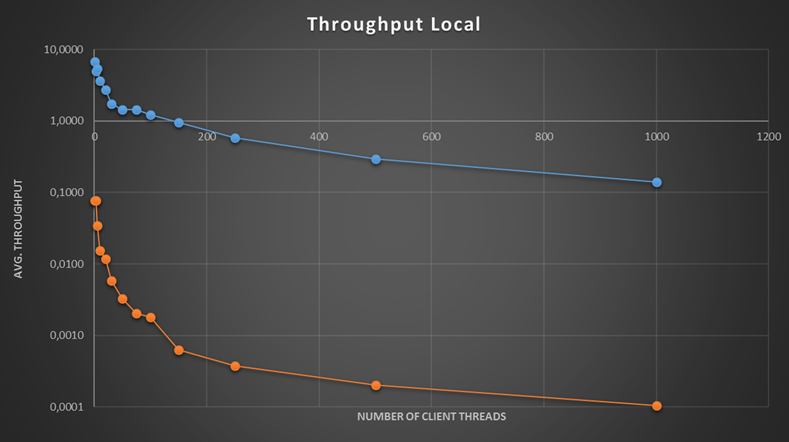
\includegraphics[scale=0.6]{throughput.png}
				\caption{Plot of average throughput using 1 to 1000 concurrent workload threads}
				\label{fig1}
		\end{figure}
		\begin{figure}
				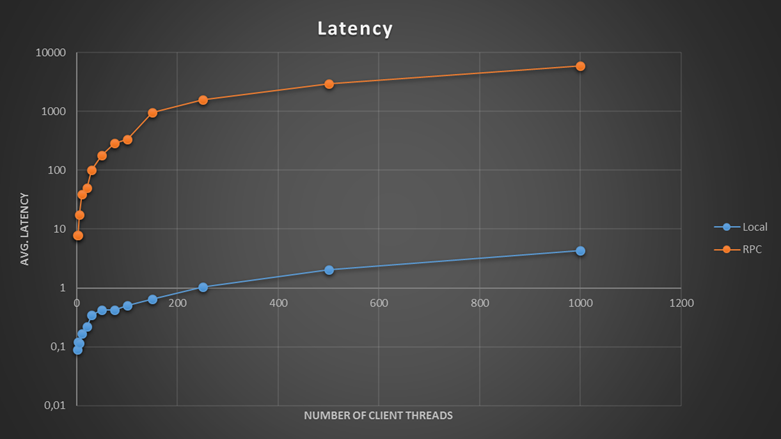
\includegraphics[scale=0.6]{latency.png}
				\caption{Plot of average latency using 1 to 1000 concurrent workload threads}				
				\label{fig2}
		\end{figure}
	\end{center}
\end{enumerate}
\end{document}